\documentclass[12pt]{article}
\usepackage{amsthm,amssymb,amsmath,amsfonts}
\usepackage[a4paper, top=25mm, bottom=30mm, left=25mm, right=25mm]{geometry}
\usepackage[pagebackref=false,colorlinks,linkcolor=black,citecolor=black]{hyperref}
\usepackage[nameinlink]{cleveref}
 \AtBeginDocument{%
    \crefname{equation}{برابری}{equations}%
    \crefname{chapter}{فصل}{chapters}%
    \crefname{section}{بخش}{sections}%
    \crefname{appendix}{پیوست}{appendices}%
    \crefname{enumi}{مورد}{items}%
    \crefname{footnote}{زیرنویس}{footnotes}%
    \crefname{figure}{شکل}{figures}%
    \crefname{table}{جدول}{tables}%
    \crefname{theorem}{قضیه}{theorems}%
    \crefname{lemma}{لم}{lemmas}%
    \crefname{corollary}{نتیجه}{corollaries}%
    \crefname{proposition}{گزاره}{propositions}%
    \crefname{definition}{تعریف}{definitions}%
    \crefname{result}{نتیجه}{results}%
    \crefname{example}{مثال}{examples}%
    \crefname{remark}{نکته}{remarks}%
    \crefname{note}{یادداشت}{notes}%
    \crefname{observation}{مشاهده}{observations}%
    \crefname{algorithm}{الگوریتم}{algorithms}%
    \crefname{cproof}{برهان}{cproofs}%
}

\usepackage{tikz}
\usepackage{graphicx}
\usepackage{booktabs}
\usepackage{color}
\usepackage{graphicx}
\usepackage{subcaption}

\usepackage{setspace}
\doublespacing

\usepackage{titletoc}
\usepackage{tocloft}
\usepackage{enumitem}
\usepackage{amsmath, amssymb}
\usepackage{algorithm}
\usepackage[noend]{algorithmic}
\renewcommand{\algorithmicrequire}{\textbf{Input:}}
\renewcommand{\algorithmicensure}{\textbf{Output:}}

\usepackage{tabularx}
\makeatletter
\newcommand{\multiline}[1]{%
  \begin{tabularx}{\dimexpr\linewidth-\ALG@thistlm}[t]{@{}X@{}}
    #1
  \end{tabularx}
}
\makeatother

\usepackage{float}
\usepackage{verbatim}
\makeindex
\usepackage{sectsty}
\usepackage{xepersian}
\SepMark{-}
\settextfont[Scale=1.2,Path=fonts/,BoldFont=B Nazanin Bold.ttf]{B Nazanin.ttf}
\setlatintextfont{Times New Roman}
\renewcommand{\labelitemi}{$\bullet$}

\theoremstyle{definition}
\newtheorem{definition}{تعریف}[section]
\newtheorem{remark}[definition]{نکته}
\newtheorem{note}[definition]{یادداشت}
\newtheorem{example}[definition]{نمونه}
\newtheorem{question}[definition]{سوال}
\newtheorem{remember}[definition]{یاداوری}
\newtheorem{observation}[definition]{مشاهده}
\theoremstyle{theorem}
\newtheorem{theorem}[definition]{قضیه}
\newtheorem{lemma}[definition]{لم}
\newtheorem{proposition}[definition]{گزاره}
\newtheorem{corollary}[definition]{نتیجه}
\newtheorem*{cproof}{برهان}




\begin{document}
\fontsize{12pt}{14pt}\selectfont

\begin{minipage}{0.1\textwidth}

\includegraphics[width=3cm]{etc/IUST}
\end{minipage}%
\hfill%
\begin{minipage}{0.6\textwidth}\centering
\fontsize{13pt}{13pt}\selectfont
به‌ نام خدا \\
\textbf{درس یادگیری عمیق} \\
\textbf{تمرین سری ششم}\\
استاد درس : دکتر محمدرضا محمدی \\
دستیاران :  مهدی خورشا، سید محمد موسوی،\\ امیرحسین نمازی
\\
\vspace{0.25cm}
\begingroup
\fontsize{11pt}{11pt}\selectfont
دانشگاه علم و صنعت ایران، دانشکده مهندسی کامپیوتر \\
نیمسال دوم تحصیلی 1403 - 1404 \\
\endgroup
\end{minipage}%
\hfill%
\begin{minipage}{0.1\textwidth}

\end{minipage}

\vspace{0.5cm}

\noindent\rule{\textwidth}{1pt}

\centering {\fontsize{18}{22}\selectfont \textbf{مهلت تحویل : 1404/02/05 }}\\
{\fontsize{14}{22}\selectfont \textbf{لطفا به نکات موجود در سند قوانین انجام و تحویل تمرین ها دقت فرمایید. }}

\begin{enumerate}

    \section*{سوالات تئوری}
    \item 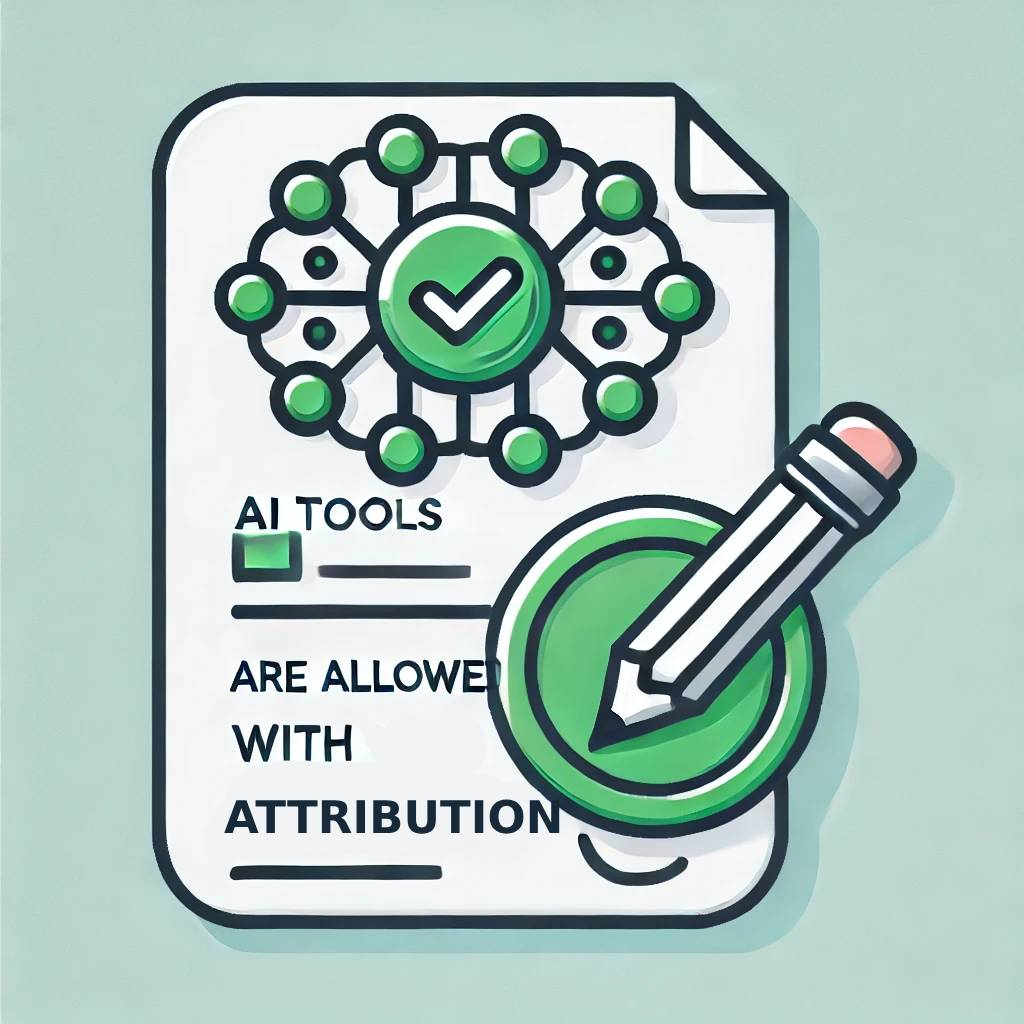
\includegraphics[width=1cm]{figs/Allowed_with_contributino.jpg}
     از مدل‌های \lr{Sequence-to-Sequence} برای حل مسائل مشترک بینایی ماشین و پردازش زبان مانند مسئله \lr{Video Captioning} و از نوع \lr{Many-to-Many} آنها استفاده می‌شود. در مقاله \lr{CAM-RNN}زیر برای حل این مسئله از معماری‌های \lr{CNN} و \lr{RNN} استفاده شده‌است. نحوه حل مسئله را در این مقاله توضیح دهید. آیا ایده‌ی این مقاله را برای مسئله \lr{Image Captioning} می‌توان استفاده کرد؟ توضیح دهید(10 نمره).\\
    \textcolor{blue}{
    \lr{RNN} یک متد که برای تسک \lr{video captioning} است. در آن از \lr{co-attention} به همراه \lr{RNN} استفاده شده است تا یک \lr{caption} توصیفی و دقیق تولید کنند. رویکرد های معمولی بر اساس \lr{RNN} هستند که کلمه به کلمه برای ویدیو، کپشن تولید میکنند و کلمه فعلی، بر اساس محتوای تصویر و کلمه قبلی تولید شده، تولید میشود. در \lr{CAM-RNN} از تصویر و متن، یکسری \lr{feature} تولید میشود و \lr{RNN} به عنوان \lr{decoder} عمل کرده و برای ویدیو کپشن تولید میکند. \lr{CAM-RNN} از سه ماژول تشکیل شده است: \lr{visual attention module} و \lr{text attention module} و \lr{balancing gate}. در حین تولید کپشن، \lr{visual attention} به صورت تطبیقی معلوم میکند که کدام قسمت از کدام فریم برجسته ترین است و باید به آن توجه کرد و به کدام فریم مرتبط ترین به کپشن است و باید به آن توجه کرد. \lr{Text attention module} به صورت اتوماتیک به مرتبط ترین کلمه یا \lr{phrase} تولید شده قبلی توجه میکند. علاوه بر آن بین این دو \lr{attention module} از یک \lr{balancing gate} استفاده شده است تا بتوان تاثیر هرکدام از \lr{text feature} و \lr{visual feature} را در هنگام تولید کپشن، کنترل و تنظیم کرد.
    به صورت دقیق تر این روش شامل بخش های زیر است:\\
    \begin{itemize}
        \item یک \lr{visual attention module} که شامل دو لایه است و برای استخراج ویژگی های قوی تر و بهتر استفاده شده است و مرتبط ترین فریم و برجسته ترین ناحیه در آن فریم را مشخص میکند.
        \item یک \lr{phrase-level text attention module} که در هنگام تولید کپشن، به مرتبط ترین قسمت از \lr{phrase} های تولید شده قبلی توجه میکند و میتواند \lr{text feature} های دقیق تری به دست آورد.
        \item یک \lr{balancing gate} که برای تنظیم تاثیر \lr{visual features} در هنگام فرآیند تولید کپشن است و برای تولید کلمات غیر بصری مناسب است.
    \end{itemize}
    معماری این سیستم در زیر آورده شده است:\\
    \begin{figure}[h]  
        \centering
        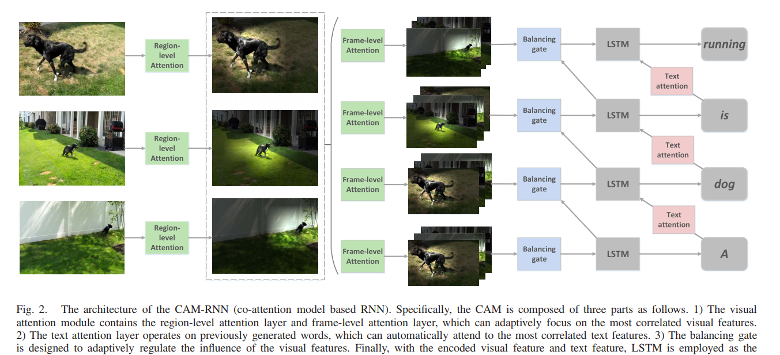
\includegraphics[width=\textwidth]{figs/Q1.png}
        \label{fig:q1}  
    \end{figure}}
    \\
    \textcolor{blue}{
    با توجه به اینکه در \lr{image captioning} میتوان تصویر را به صورت فیلمی که تنها یک فریم دارد، تصور کرد میتوان به این صورت برای آن کپشن تولید کرد ولی دیگر \lr{frame-level attention} کاربردی ندارد زیرا تنها یک فریم داریم که میتوانیم به آن توجه کنیم.
    }
    \item 
\includegraphics[width=1cm]{figs/Forbidden_AI.jpg}
    با فرض اینکه ابعاد داده ورودی 128 و ابعاد بردار نهان 64 باشد، تعداد پارامترهای یک لایه \lr{Simple RNN} و \lr{GRU} و \lr{LSTM} و \lr{BiLSTM} را با ذکر کامل جزئیات محاسبات به دست آورده و با هم مقایسه کنید(12 نمره).\\
    \textcolor{blue}{
        $$
            \begin{aligned}
            & \text {\lr{Simple RNN}}=128 * 64+64 * 64+64=8192+4096+64=12352 \\
            & \text {\lr{GRU}}=12352 * 3=37056 \\
            & \text {\lr{LSTM}}=12352 * 4=49408 \\
            & \text {\lr{BiLSTM}}=49408 * 2=98816
            \end{aligned}
        $$
    }
    
    \item 
\includegraphics[width=1cm]{figs/Forbidden_AI.jpg}
    برای حل هر یک از مسائل زیر، یک معماری مناسب از بین انواع معماری‌های \lr{RNN} که تاکنون آموخته‌اید، انتخاب کنید. معماری‌های مورد نظر شامل \lr{One-to-Many}، \lr{Many-to-One} و \lr{Many-to-Many} هستند. پس از انتخاب، دلیل خود را برای استفاده از آن معماری به‌طور واضح توضیح دهید(18 نمره).
    \begin{itemize}
        \item \lr{Text Summarization} : \textcolor{blue}{\lr{many-to-many}}
        \item \lr{Machine Translation} : \textcolor{blue}{\lr{many-to-many}}
        \item \lr{Video Captioning} : \textcolor{blue}{\lr{many-to-many}}
        \item \lr{Sentiment Analysis} : \textcolor{blue}{\lr{many-to-one}}
        \item \lr{Automatic Speech Recognition} : \textcolor{blue}{\lr{many-to-many}}
        \item \lr{Question Answering} : \textcolor{blue}{\lr{many-to-many, many-to-one}}
        \item \lr{Text-to-Speech} : \textcolor{blue}{\lr{many-to-many}}
        \item \lr{Paraphrase Generation} : \textcolor{blue}{\lr{many-to-many}}
        \item \lr{Code Translation} : \textcolor{blue}{\lr{many-to-many}}

    \end{itemize}
    \section*{سوال امتیازی}
    \item 
\includegraphics[width=1cm]{figs/Forbidden_AI.jpg}
    با توجه به شبکه نشان‌داده‌شده در شکل زیر، به سوالات مطرح‌شده پاسخ دهید. برای سادگی، فرض کنید تمام مقادیر شامل ورودی‌ها، وزن‌ها و خروجی‌ها اسکالر هستند. همچنین تمام توابع فعال‌ساز را از نوع سیگموید \lr{σ} در نظر بگیرید(20 نمره).
    \begin{figure}[h]  
        \centering
        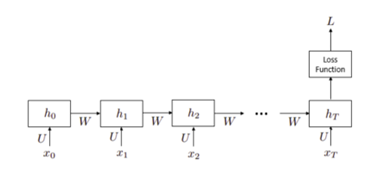
\includegraphics[width=0.85\textwidth]{figs/Q4.png}
        \label{fig:num_pic}  
    \end{figure}

    \begin{itemize}
        \item ابتدا گرادیان \lr{$h_{t}$} را بر حسب گرادیان \lr{$h_{(t+1)}$} بنویسید.\\
        \textcolor{blue}{
        $$
            \begin{aligned}
            &\begin{gathered}
            h_{t+1}=\sigma\left(U x_{t+1}+W h_t\right) \\
            \frac{\partial L}{\partial h_t}=\frac{\partial L}{\partial h_{t+1}} \frac{\partial h_{t+1}}{\partial h_t}=\frac{\partial L}{\partial h_{t+1}} \sigma^{\prime}\left(U x_{t+1}+W h_t\right) \cdot W
            \end{gathered}
            \end{aligned}
        $$
        }
        \item 	حال با استفاده از رابطه قسمت قبل، و با قاعده مشتق زنجیری، گرادیان \lr{$h_{0}$} را بر حسب گرادیان \lr{$h_{T}$} بنویسید.\\
        \textcolor{blue}{
        $$
            \begin{aligned}
            & \frac{\partial L}{\partial h_0}=\frac{\partial L}{\partial h_T} \frac{\partial h_T}{\partial h_{T-1}} \ldots \frac{\partial h_2}{\partial h_1} \frac{\partial h_1}{\partial h_0} \\
            & =\frac{\partial L}{\partial h_T}\left(\sigma^{\prime}\left(U x_T+W h_{T-1}\right) \cdot W\right) \ldots\left(\sigma^{\prime}\left(U x_2+W h_1\right) \cdot W\right)\left(\sigma^{\prime}\left(U x_1+W h_0\right) \cdot W\right)
            \end{aligned}
        $$
        }
        \item برش گرادیان توسط مقدار و توسط اندازه را توضیح دهید. برتری برش توسط اندازه را به برش توسط مقدار توضیح دهید.\\
        \textcolor{blue}{
        در برش توسط مقدار ما یک آستانه مانند\lr{T} در نظر گرفته و هر عنصر در بردار گرادیان که بزرگتر از\lr{T} باشد را به\lr{T} کاهش می‌دهیم. عناصر دیگر بدون تغییر باقی می‌مانند. در برش توسط اندازه ما نیز با یک آستانه مانند\lr{T} این‌بار برروی اندازه بردار گرادیان قرار داده، و اگر اندازه بردار گرادیان بیشتر از\lr{T} باشد، بردار گرادیان را طوری نرمال کرده که اندازه آن برابر\lr{T} شود. در برش توسط مقدار، چگونگی جهت بردار گرادیان در برخی جهات تقطیع کرده و در برخی دیگر از جهات نگه‌می‌داریم، این کار باعث می‌شود بردار گرادیان نهایی در جهت بردار گرادیان ابتدایی نباشد در حالی که در برش توسط اندازه چون تمام عناصر گرادیان به یک اندازه \lr{scale} می‌شوند، این اتفاق رخ نخواهد داد.
        }
    \end{itemize}
    	
    \section*{سوالات عملی} 
    \item 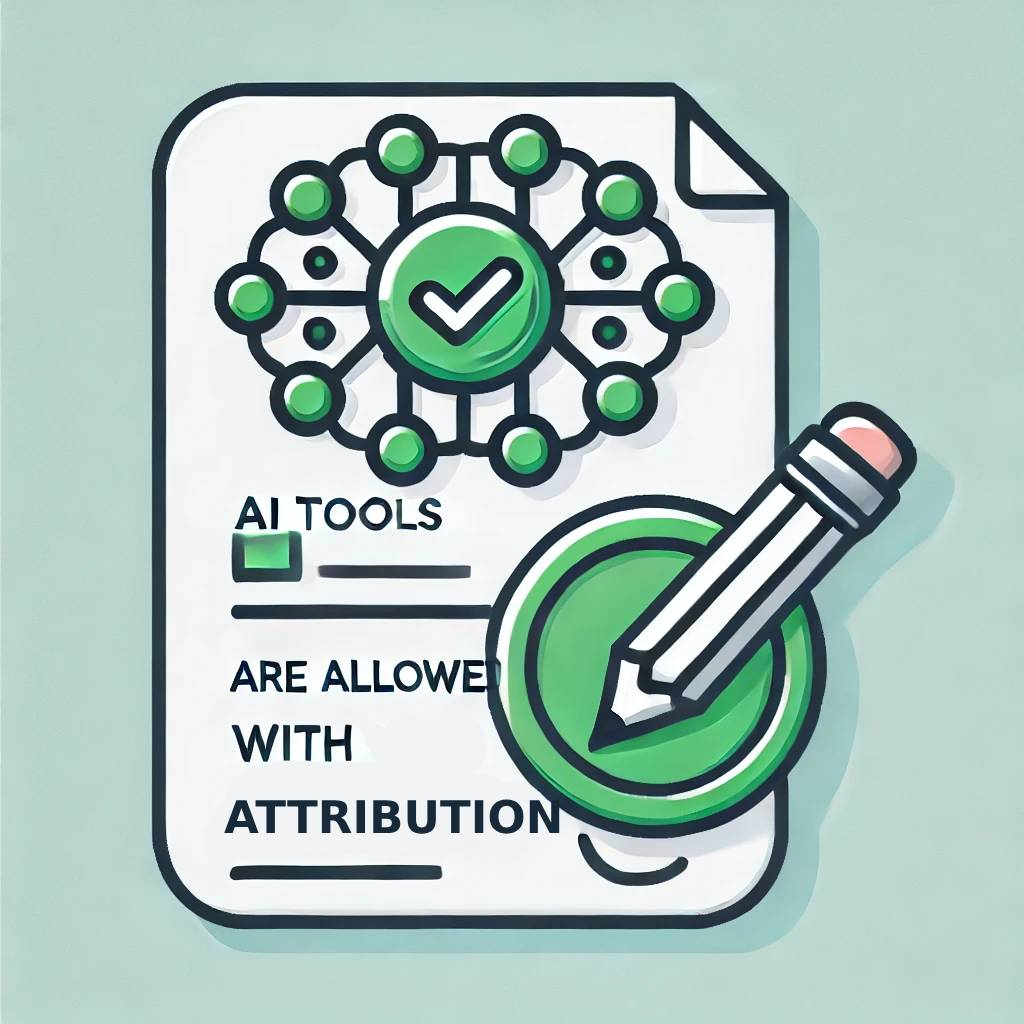
\includegraphics[width=1cm]{figs/Allowed_with_contributino.jpg}
    به نوت‌بوک \lr{divan\_hafez.ipynb} مراجعه کرده و قسمت های مشخص شده را کامل کنید. در این نوت‌بوک قرار است با استفاده از یک \lr{RNN}  متن های مشابه با غزل‌های دیوان حافظ تولید کنید(30 نمره). \\
    \textbf{در نظر داشته باشید تنها اجازه ویرایش قسمت های مشخص شده را دارید.}\\
    \textcolor{blue}{
    به نوتبوک \lr{divan\_hafez.ipynb} مراجعه کنید.
    }

    \item 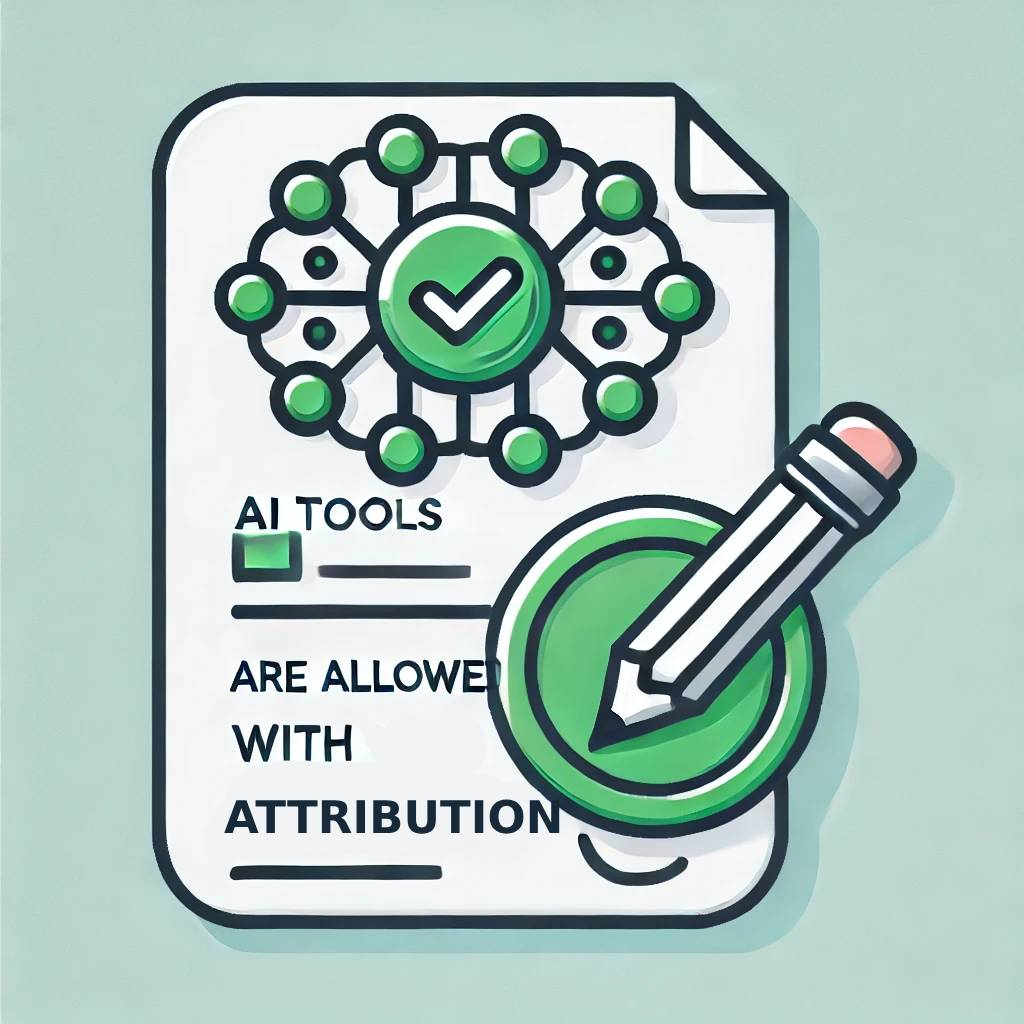
\includegraphics[width=1cm]{figs/Allowed_with_contributino.jpg}
    در سالهای اخیر توجه به رمزارزها بسیار گسترش یافته است. یکی از معروفترین رمزارزهای موجود در بازار \lr{Bitcoin} است. در این سوال قصد داریم قیمت \lr{Bitcoin} را در آینده پیش‌بینی کنیم. برای این کار مراحل زیر را دنبال نمایید(30 نمره).\\
    \begin{itemize}
        \item   ابتدا لازم است کتابخانه \lr{yfinance} را نصب نمایید. این کتابخانه را میتوانید به کمک این \href{https://pypi.org/project/yfinance/}{لینک} نصب نمایید.
        \item   حال میتوانید قیمت \lr{Bitcoin} را دانلود نمایید. برای این کار از تابع \lr{download} موجود در این \href{https://github.com/ranaroussi/yfinance}{لینک} استفاده کنید. لازم به ذکر است نماد شاخص مورد نظر برابر با \lr{BTC-USD} است و تاریخ ذخیره‌سازی برای داده‌های آموزشی را برابر با \lr{0.8} ابتدایی داده ها از لحاظ زمانی قرار دهید.
        \item برای آزمایش درستی مراحل فوق، نمودار این شاخص را بر حسب زمان رسم نمایید و به هر یک از داده‌های آموزشی و آزمایشی رنگ متفاوتی اختصاص دهید. نمودار حاصل مشابه با نمودار زیر خواهد بود.
        \begin{figure}[h]  
            \centering
            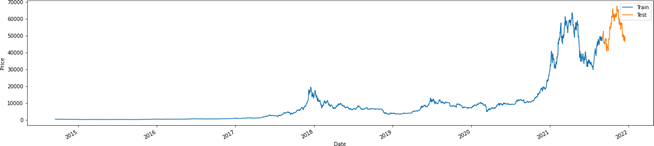
\includegraphics[width=\textwidth]{figs/Q6_1.png}
            \label{fig:num_pic}  
        \end{figure}
        \item   مقادیر محور \lr{y} نمودار فوق را با استفاده از تابع \lr{MinMaxScaler} کتابخانه \lr{scikit-learn} نرمالیزه کنید. توجه داشته باشید تنها از داده‌های آموزشی برای تنظیم مقیاس استفاده کنید و داده‎‌های آزمون را براساس معیار داده‌های آموزش مقیاس‌شان تنظیم می‌شود.
        \item   در مرحله بعد داده‌های مورد نیاز برای آموزش و آزمایش مدل را تهیه می‌نماییم. برای این کار متغیری تعریف کنید که نشان دهنده تعداد داده‌های گذشته برای پیش‌بینی داده مشخصی باشد. به عنوان مثال اگر این متغیر را برابر با 60 قرار دهید، یعنی از 60 داده گذشته در پیش‌بینی آن داده استفاده شده‌است.
        \item   مدل را مشابه با معماری شکل زیر بسازید.
        \begin{figure}[h]  
            \centering
            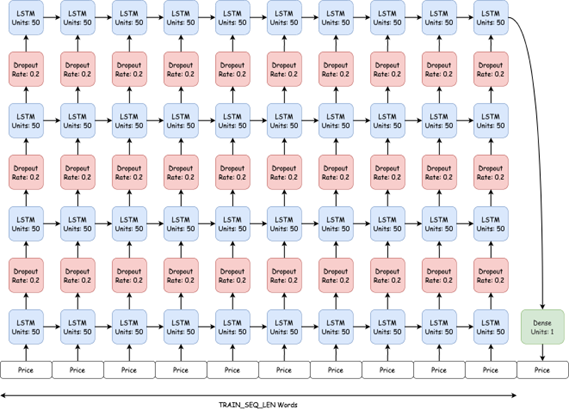
\includegraphics[width=0.95\textwidth]{figs/Q6_2.png}
            \label{fig:num_pic}  
        \end{figure}
        \item   حال این مدل را با بهینه‌ساز \lr{AdamW} و تابع ضرر \lr{MSE} و \lr{BatchSize=32} به تعداد 100 ایپاک آموزش دهید.
        \item   پس از آموزش مدل، پیش‌بینی را بر روی داده‌های آزمون انجام دهید و نمودار را رسم نمایید. در این نمودار که بر حسب زمان رسم می‌شود، هر دو مقدار واقعی و پیش‌بینی را با رنگ‌های متفاوت رسم کنید.
        \item   در نهایت، به صورت متوالی آینده را از زمانی که داده‌ها به پایان می‌رسند پیش‌بینی کنید.
        \item   افزایش یا کاهش متغیر تعریف شده در مرحله تهیه داده مورد نیاز برای آموزش مدل یعنی تعداد داده‌های گذشته برای پیش‌بینی داده‌های مشخص چه مزایا یا معایبی دارد؟ شرح دهید.
        
    \end{itemize}
    \textcolor{blue}{
    به نوتبوک \lr{bitcoin\_price\_prediction\_lstm\_pytorch.ipynb} مراجعه کنید.
    }

\end{enumerate}



\end{document}


